\chapter{Calculation Details to Chapter 4}
\section{Model system}\label{chap03:sec:appa}

In this Appendix, we shall briefly justify Eqs.~(\ref{chap03:eff}) and (\ref{chap03:full}) of the main text. We start from an $s$-$d$-like model for two-dimensional antiferromagnet on a honeycomb lattice \cite{sumit2019}. The model includes a local exchange interaction between localized magnetic moments and conduction electron spins as given by Eq.~(\ref{chap03:ex}). Itinerant electrons in the model are, therefore, governed by the tight-binding Hamiltonian 
\begin{align}
H_0=\,&-t\sum\limits_{i}\s_{\sigma\sigma'}c_{i\sigma}^\dagger c_{i\sigma'}
-J \s_{i} \s_{\sigma\sigma'}\bb{S}_i\cdot \bb{\sigma}_{\sigma\sigma'}c^\dagger_{i\sigma}c\0_{i\sigma'}\n+\frac{i\lambda}{3a}\s_{\langle i,j\rangle}\sum\limits_{\sigma\sigma'}\hat{\bm{z}}\cdot(\bm{\sigma}\times\bm{d}_{ij})_{\sigma\sigma'}c_{i\sigma}^\dagger c_{j\sigma'},
\label{chap03:htb}
\end{align}
where we do ignore disorder for a moment. The model is characterized by the nearest neighbor hopping energy $t$ and the Rashba spin-orbit coupling energy $\lambda$, $z$-axis is aligned perpendicular to the two-dimensional plane, the in-plane vectors $\bm{d}_{ij}$ connect the neighboring sites $i$ and $j$ on a honeycomb lattice. For any site $i$ on the sublattice $A$ we choose
\be
\bb{d}_{1}= a \bpm 0 \\ 1 \epm, \quad \bb{d}_{2}= \frac{a}{2} \bpm \sqrt{3} \\ -1 \epm , \quad \bb{d}_{3}= -\frac{a}{2} \bpm \sqrt{3}  \\ 1 \epm,
\e
where $a$ is the length of the bond between $A$ and $B$.

By projecting the tight-binding model of Eq.~(\ref{chap03:htb}) on states in a vicinity of the valley wave-vectors,
\be
\bb{K}= \frac{4\pi}{3\sqrt{3} a}\bpm 1\\ 0\epm,\quad\mbox{and}\quad \bb{K}'= -\bb{K},
\e
we find, in the valley symmetric approximation, the effective Hamiltonian of Eq.~(\ref{chap03:eff}) with the assumption that $\bb{S}^A=-\bb{S}^B$, where $v = 3ta/2\hslash$. By relaxing the assumption we obtain the model of Eq.~(\ref{chap03:full}).

\section{Linear Response tensors}\label{chap03:sec:appb}
\label{chap03:app:vertexcorrections}
In order to keep technical expressions compact we let $\hslash=1$ and $\ep_F=\ep$ below. Our technical analysis is based on linear response of electron spin density to various perturbations at zero frequency ($dc$) limit. In particular, we consider three types of responses: the one with respect to electric current (via electric field and inverse conductivity tensor), the one with respect to the time derivative of the N\'eel vector 
and the other one with respect to the time derivative of magnetization vector. These responses are summed up as
\beml
\label{chap03:tensors}
\begin{align}
\delta\bb{s}^+=\hat{S}^\textrm{SOT}_+\bb{j} +\hat{S}^\textrm{GD}_{mn} \dot{\bb{n}}+\hat{S}^\textrm{GD}_m\dot{\bb{m}},\\
\delta\bb{s}^-=\hat{S}^\textrm{SOT}_-\bb{j}+\hat{S}^\textrm{GD}_{nm}\dot{\bb{m}}+\hat{S}^\textrm{GD}_n \dot{\bb{n}},
\end{align}
\eml
where we define the response tensors $\hat{S}^\textrm{SOT}_\pm$ that are describing spin-orbit torques (both field-like and anti-damping) and various $\hat{S}^\textrm{GD}$ tensors that are describing various contributions to Gilbert dampings (and to effective spin renormalizations) \cite{ado_anisotropy_2019}.

In order to compute the linear response tensors in Eqs.~(\ref{chap03:tensors}) we apply the standard Kubo formula (see Appendix~\ref{kubo})
\be
\label{chap03:chap3:eq:kubo}
\delta\bb{s}^\pm_\alpha = 
\frac{J^2Sv^2\mathcal{A}}{2 V}
\s_\beta \widehat{\tr}  \lt\la \hat{G}^\text{R} \hat{s}^\pm_\alpha \hat{G}^\text{A}  
\hat{F}_\beta \rt\ra \,\frac{\pa X_\beta}{\pa t},
\e
where $V$ is the system area, $\widehat{\tr}$ is an operator trace, $\hat{G}^\text{R(A)}=(\ep-H\pm i 0)$ are retarded (advanced) Green function operators, $\hat{s}_\alpha^+ = \sigma_\alpha$, $\hat{s}_\alpha^-=\Lambda_z\Sigma_z\sigma_\alpha$ are the operators corresponding to the average spin-polarization $\bb{s}^+$ and staggered spin-polarization $\bb{s}^-$, the product $\hat{\bb{F}}\cdot \bb{X}(t)$ represents the time-dependent perturbation in the Hamiltonian, while the angular brackets denote the disorder averaging that we consider in diffusive (ladder) approximation.

The linear-response formula Eq.~(\ref{chap03:chap3:eq:kubo}) assumes zero temperature and zero frequency limit that corresponds to taking both Green's functions at the same energy $\ep=\ep_F$. We also neglect the Fermi-sea contribution (also known as St\v{r}eda contribution) since such a contribution appears to be either zero or subleading in the metal parameter $\ep\tau\gg 1$ with respect to our results.  
 
Thus, in order to compute Gilbert dampings and spin-orbit torque tensors we consider linear response of $\delta\bb{s}^\pm$ to the three perturbations mentioned above. Each perturbation is parameterized by the term $\delta H=\hat{\bb{F}}\cdot \bb{X}(t)$ with
\beml
\label{chap03:chap3:eq:ops}
\begin{align}
&\dot{\bb{X}}=\dot{\bb{n}},\qquad \hat{\bb{F}}=-\Delta\,\Lambda_z\Sigma_z\bb{\sigma},\\ 
&\dot{\bb{X}}=\dot{\bb{m}},\qquad\qquad\hat{\bb{F}}=-\Delta\, \bb{\sigma},\\
&\dot{\bb{X}}=(\pi v/e)\hat{\sigma}^{-1}\bb{j},\quad \hat{\bb{F}} =\bb{\Sigma},
\end{align}
\eml
where $\hat{\sigma}$ is the conductivity tensor (this is computed from the standard Kubo formula which is analogous to the one in Eq.~(\ref{chap03:chap3:eq:kubo}) but for the response of current density to electric field). The disorder averaging amounts to replacing Green's functions in Eq.~(\ref{chap03:chap3:eq:kubo}) with the corresponding disorder-averaged Green's functions and to replacing one of the operators, $\hat{s}_\alpha$ or $\hat{F}$, with the corresponding vertex-corrected operator.

Disorder-averaged Green's functions become diagonal in the momentum space due to restored translational invariance and take the form 
$G^\text{R(A)}_{\bb{p}} = [\ep-H-\Sigma^\textrm{R(A)}]^{-1}$, where the Hamiltonian $H$ is defined in Eq.~(\ref{chap03:eff}) of the main text, while the self-energy $\Sigma^\text{R(A)}$ is evaluated in the Born-approximation depicted schematically in Fig.~\ref{chap03:fig:diagrams}a. 

We find that the real part of the self-energy does renormalize the Fermi energy $\ep$ and the $s$-$d$ exchange coupling strength $\Delta$, while the imaginary part reads
\be
\im \Sigma^\text{R(A)} = \mp\frac{\pi\alpha_d}{2}\,(\ep-\Delta\,\Lambda_z\Sigma_z\,\bb{n}\cdot\bb{\sigma}).
\e

\begin{figure}
\centering
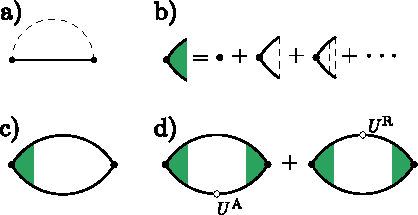
\includegraphics{articles/misha_paper/app5.pdf}
\caption{Diagrammatic illustration. a) Born-approximation. b) Ladder-approximation. c) Disorder-averaged polarization bubble. d) Perturbative expansion of the disorder-averaged polarization bubble. }
\label{chap03:fig:diagrams}
\end{figure}

In order to evaluate linear response tensors in the leading order with respect to the metal parameter $\ep\tau \gg 1$ one also needs to sum up the ladder diagrams as shown in Fig.~\ref{chap03:fig:diagrams}b-c. Refering to Chapter~\ref{diagrammatics}, 
we first need to define the vertex corrected operator
\be
\label{chap03:chap3:eq:ladder}
\hat{F}^\text{vc}= \hat{F}+\hat{F}^{(1)} +\hat{F}^{(2)}+\hat{F}^{(3)}+\cdots,
\e
where we denote by $\hat{F}^{(i)}$ the operator $\hat{F}$ that is dressed by the number of $i$ disorder lines,
\be
\label{chap03:chap3:eq:onedisorderline}
\hat{F}^{(i)} = 2\pi\alpha_d\int\frac{\mathrm{d}^2\bb{p}}{(2\pi)^2} G_{\bb{p}}^\text{R}\hat{F}^{(i-1)}G_{\bb{p}}^\text{A}. 
\e
A suitable basis to work in is 
\be
B_i=\frac{1}{2}\Lambda_\zeta\Sigma_\alpha \sigma_\beta,\quad i=\{\zeta,\alpha,\beta\},
\e
where $i$ is a cumulative index with $\zeta =0,z$ a valley parity index and $\alpha, \beta$ taking on the four values $\{0,x,y,z\}$ each. 

For $\bb{B}=(B_1, B_2,\dots, B_{32})$ we define the vertex corrected operator vector as 
\be
\label{chap03:sum}
\bb{B}^{\text{vc}}=\bb{B}+\mathcal{F}\bb{B}+\mathcal{F}^2\bb{B}+\mathcal{F}^3\bb{B}+\dots=
\frac{1}{1-\mathcal{F}}\bb{B},
\e
where $\mathcal{F}$ stands for a matrix of vertex corrections. Using the normalization condition $\tr B_i B_j =2\delta_{ij}$ 
we find
\be
\label{chap03:chap3:eq:matrixF}
\mathcal{F}_{ij} = \pi\alpha_d \int \frac{\mathrm{d}^2\bb{p}}{(2\pi)^2} 
\tr \lt[G^\text{A}_{\bb{p}} B_i G^\text{R}_{\bb{p}} B_j\rt],
\e
where $\tr$ stands for the usual matrix trace in the valley, spin and sublattice spaces.   

We note that the matrix $\mathcal{F}$ is evidently diagonal in the valley space, and it can also become block-diagonal in sublattice and spin spaces by choosing a more convenient basis. 

A particularly useful choice of basis corresponds to in-plane rotation of both spin and sublattice Pauli matrices to the frame associated with the in-plane projection $\bb{n}_\parallel$ of the N\'eel vector. For spin Pauli matrices this transformation is given by
\be
\label{chap03:trans}
\sigma_x \rightarrow \Lambda_z\frac{n_x \sigma_x + n_y \sigma_y }{\sqrt{n_x^2+n_y^2}}, \quad \sigma_y \rightarrow \Lambda_z\frac{n_y \sigma_x - n_x \sigma_y }{\sqrt{n_x^2+n_y^2}},
\e
where we took advantage of the fact that the direction of $\bb{n}$ is opposite in the two valleys. The same transformation (\ref{chap03:trans}) has to be applied to $\Sigma_{x}$ and $\Sigma_{y}$. 

The matrix $\mathcal{F}$ is instrumental for the analysis of all linear response tensors in Eq.~(\ref{chap03:tensors}). Indeed, using the definition of Eq.~(\ref{chap03:chap3:eq:matrixF}) in Eq.~(\ref{chap03:chap3:eq:kubo}) and summing up the diffusion ladders we find
\be
\label{chap03:final}
\delta s^\pm_\alpha = \frac{J^2S v^2\mathcal{A}}{2 \pi \alpha_d}
\s_\beta \s_{ij} \tr[\hat{s}^\pm_\alpha B_i] \mathcal{R}_{ij} \tr[\hat{F}_\beta B_j] \,\frac{\pa X_\beta}{\pa t},
\e
where $\mathcal{R}=\mathcal{F}(1-\mathcal{F})^{-1}$. Thus, the computation of all response tensors is reduced in the diffusive approximation to the computation of the vertex correction matrix $\mathcal{F}$ and subsequent matrix inversion.  

\section{Vertex correction}\label{chap03:sec:appc}

Still, finding an inverse matrix $(1-\mathcal{F})^{-1}$ is not that straightforward due to a pair of eigenvalues (one per valley) that equal exactly $1$. The presence of such eigenvalues roots in the particle conservation and is, therefore, not an artificial problem. The unit eigenvalues do evidently prevent the matrix inversion in Eq.~(\ref{chap03:sum}). Nevertheless, it can be shown that the corresponding eigenvectors do not enter the final equations of motion for localized spins. In the next section, we briefly illustrate how one can formally avoid the particle conservation divergence in the computation of vertex corrections.

Let us define by $\bb{a}_\zeta$ the eigenvectors of $\mathcal{F}$ that correspond to two unit eigenvalues, $\mathcal{F}\bb{a}_\zeta=\bb{a}_\zeta$, with $\zeta=0, z$. For the  normalized vector $\bb{a}_\zeta$ we define special operators
\be
\label{chap03:Bdiv}
\bar{B}_\zeta=\bb{a}_\zeta \cdot \bb{B} 
= \frac{\varepsilon-\Delta \Lambda_\zeta \Sigma_z\,\bm{n}\cdot\bm{\sigma}}{2\sqrt{\varepsilon^2+\Delta^2}},
\e
which are conserved with respect to impurity dressing $\bar{B}_\zeta=\bar{B}_\zeta^{(i)}$ for any order $i$. This means that the vertex corrected operator $\bar{B}_\zeta^\textrm{vc}$ is formally diverging in the $dc$ limit. In what follows, we formally write $\bar{B}_\zeta^{\text{vc}} = R_\infty \bar{B}_\zeta$, where the limit $R_\infty \to \infty$ is taken at the end of the calculation.

The response tensors defined by Eqs.~(\ref{chap03:response}) consist of different correlators of the operators $\Sigma_\alpha$, $s^+_\alpha=\sigma_a$, and $s^-_\alpha = \Lambda_z\Sigma_z\sigma_\alpha$. It is evident that most of these operators are already orthogonal to $\bar{B}_\zeta$,
\be
\tr \lt[\Sigma_\alpha \bar{B}_\zeta\rt] = \tr \lt[s^+_\alpha \bar{B}_\zeta\rt]= \tr \lt[s^-_\alpha \bar{B}_0\rt] =0,
\e
while the only dangerous sector is related to the projection
\be
\label{chap03:finite}
\tr \lt[s^-_\alpha \bar{B}_z\rt] = - \frac{4\Delta\, n_\alpha}{\sqrt{\varepsilon^2+\Delta^2}},
\e
which is evidently finite. The result of Eq.~(\ref{chap03:finite}) leads to formally diverging contribution $\delta \bb{s}^-_\textrm{div}$ that is generally present in all components of $\delta \bb{s}^-$, 
\be
\delta s^{-}_{\textrm{div},\alpha}\propto  R_\infty
\s_\beta \tr[\hat{\bb{s}}_\alpha^- \bar{B}_z] \tr[\hat{F}_\beta \bar{B}_z] \,\frac{\pa n_\beta}{\pa t}.
\e
One can immediately see, however, that such a diverging contribution corresponds to a particular vector form,
\be
\label{chap03:divergence}
\delta s^{-}_{\textrm{div},\alpha} \propto R_\infty n_\alpha\, \bb{n}\cdot\frac{\pa \bb{n}}{\pa t} =0,
\e
that manifestly vanishes due to the constraint $|\bb{n}|=1$ which is exact in the limit $\bb{m}=0$. Thus, the divergency in $B_\textrm{div}^\textrm{vc}$ (which originates in the diffusion pole of the density-density response) is, in fact, harmless for the response 
tensors we are discussing. 

It is interesting to note that the irrelevance of the divergency in $B_\textrm{div}^\textrm{vc}$ operator extends to higher orders in $\bb{m}$, even though it becomes much harder to see. We touch on this problem in Appendix~\ref{chap03:sec:appd}. 

\section{Finite magnetization}\label{chap03:sec:appd}
The deviation from a collinear antiferromagnetic order can be accounted by considering a finite net magnetization term in the Hamiltonain perturbatively,
\be
H =H^\textrm{eff}+ U, \qquad U = -\Delta\,\bb{m}\cdot\bb{\sigma}.
\e
In the paper, we build the first order perturbation theory with respect to $U$. 

First of all, it can be shown that the self-energy acquires the linear in $\bb{m}$ contribution as
\be\label{chap03:chap3:eq:SEcorr}
\im \Sigma^\text{R(A)} = \mp\frac{\pi\alpha_d}{2}\,(\ep-\Delta\,\Lambda_z\Sigma_z\,\bb{n}\cdot\bb{\sigma}+\Delta\,\bb{m}\cdot\bb{\sigma}).
\e
Second, the Dyson expansion of the disorder-averaged Green's functions $G^\text{R(A)}$ with respect to $\bb{m}$ reads
\be
G^\text{R(A)}\rightarrow G^\text{R(A)}+G^\text{R(A)}U^\text{R(A)}G^\text{R(A)},
\e
where $U^\text{R(A)}=U(1 \pm i \pi\alpha_d/2)$ and we disregarded terms starting from quadratic order in $\bb{m}$. Note, that 
we have kept the notations $G^\text{R(A)}$ for the disorder averaged Green's functions of the unperturbed system. 

The computation of linear response tensors amounts to considering an additional contribution to the response tensor represented by a complex class of diagrams depicted schematically in  Fig.~\ref{chap03:fig:diagrams}d. Before ladder summation is applied the diagrams of Fig.~\ref{chap03:fig:diagrams}d correspond to a contribution to the correlator of two operators $B_i$ and $B_j$ of the type 
\begin{align}
\mathcal{U}_{ij} = 2\pi\alpha_d \int \frac{d^2\bb{p}}{(2\pi)^2} \tr\lt[G^\text{A} U^\text{A} G^\text{A} B_i G^R B_j\n+G^\text{A} B_i G^R U^R G^R B_j\rt],   
\end{align}
which has yet be dressed. The dressing amounts to replacing both $B_i$ and $B_j$ operators with the corresponding vertex corrected operators $B^\textrm{vc}_i$ and $B^\textrm{vc}_j$, respectively. 

The final result for the response of spin density is still given by Eq.~(\ref{chap03:final}), where the matrix $\mathcal{R}=\mathcal{F}(1-\mathcal{F})^{-1}$ is, however, replaced with 
\be
\label{chap03:chap3:eq:mresp}
\mathcal{R}=\frac{\mathcal{F}}{1-\mathcal{F}} + \frac{1}{1-\mathcal{F}}\mathcal{U}\frac{1}{1-\mathcal{F}},
\e
which corresponds to diagrams Fig.~\ref{chap03:fig:diagrams}c-d.
It is again convenient to consider a particular basis for the matrix $\mathcal{F}$ as defined in Eq.~(\ref{chap03:trans}) to simplify analytical computation.  

The problem of divergence in the operators $\bar{B}_\zeta$ does now become less trivial. Careful analysis shows that the linear terms in $\bb{m}$ included in Eq.~(\ref{chap03:chap3:eq:mresp}) lead to additional diverging contributions to $\delta\bb{s}^{-}$ of the form
\be
\label{chap03:extra}
\delta\bb{s}^{-, (1)}_{\text{div},\alpha} \propto  - R_\infty n_\alpha\, \bb{m}\cdot\frac{\pa \bb{m}}{\pa t},
\e
that is analogous to the one in Eq.~(\ref{chap03:divergence}) for a finite $m$. (We remind that the constraint $n^2+m^2=1$ provides a relation between these terms). The contribution in Eq.~(\ref{chap03:extra}) is, however, of too high order in $\bb{m}$ in Eq.~(\ref{chap03:ndot}) and cancels out completely in Eq.~(\ref{chap03:mdot}).

The terms linear in $\bb{m}$ are also responsible for diverging contributions in $\delta s_\alpha^{+}$ of the type 
\be
\delta s^{+}_{\text{div},\alpha} \propto R_\infty m_\alpha\, \bb{n}\cdot\frac{\pa \bb{n}}{\pa t}= - R_\infty m_\alpha\, \bb{m}\cdot\frac{\pa \bb{m}}{\pa t},
\e
that appear to be of higher than a linear order in $\bb{m}$, thus, exceeding our working precision.

Overall, one can show that the operators $\bar{B}_\zeta$ can be formally excluded by projecting the operator space of $B_i$ operators on the corresponding subspace. The latter is facilitated by the transformation $\mathcal{F}\to P\mathcal{F}P$, where 
\be
\label{chap03:PPP}
P= 1- \s_{\zeta=0,z}\bb{a}_\zeta \bb{a}\h_\zeta, 
\e
is the projection operator. Here, $\bb{a}$ stands for the column vector and $\bb{a}\h$ for the corresponding conjugated string vector. Eq.~(\ref{chap03:PPP}) facilitates the regularized computation of the vertex corrections and lead to the results presented in the paper.